% Allow relative paths in included subfiles that are compiled separately
% See https://tex.stackexchange.com/questions/153312/
\providecommand{\main}{..}
\documentclass[\main/thesis.tex]{subfiles}

\begin{document}

\chapter{Autoencoder Embeddings with Improved Tree Ensemble}
\chaptermark{AENCXGB}
\label{chp:aencxgb}

In Chapter~\ref{chp:dl_autoenc} I discover that the autoencoder classification models provide worse overall challenge metrics compared to the gradient boosted tree model proposed in Chapter~\ref{chp:xgbensemble}, but are more sensitive in detecting \gls{irbbb}, \gls{lanfb}, and \gls{rad}.

This chapter explores the effectiveness of combining the autoencoder learned embeddings with the manually engineered features to train a new set of gradient boosted tree models.
I extend the approaches used in Chapters~\ref{chp:xgbensemble} and \ref{chp:dl_autoenc} with the following research questions:
\begin{itemize}
    \item For the shallow classification ensemble using manual feature engineering, the top $1,000$ features used were averaged across all classifier labels. Will selecting top features with respect to the label-wise classifier improve classification scoring metrics?
    \item We have a deep learning approach for generating a fixed size embedding representation of a variable length \gls{ecg} record. Will incorporating the sequence embeddings from our deep learning autoencoder improve classification scoring metrics?
    \item What are the new distributions of important feature categories for these new classifiers, with respect to each diagnosis?
\end{itemize}

\section{Methodology}

An initial processing step to convert the variable length features into fixed length input vectors is first applied on all \gls{ecg} records.
We combine the techniques applied in Section~\ref{ssec:xgb_feature_engineering} and Section~\ref{ssec:aenc_seq_embedding} to create different experiment configurations for comparison.

We propose six different experiment configurations:
\begin{enumerate}
    \item \label{item:xgb_aenc_model_1} \textbf{All Features with Embeddings}: We combine the feature engineering input vector (size 18,950) with the autoencoder sequence embedding vector (size 768) to create a combined input vector of size 19,718 and train an XGBClassifier for each of the 27 diagnosed labels.
    \item \label{item:xgb_aenc_model_2} \textbf{All Features}: We use the feature engineering input vector of size 18,950 as the input to our label-wise XGBClassifier ensembles.
    \item \textbf{Top 1000 Features with Embeddings}: Starting from Configuration~\ref{item:xgb_aenc_model_1}, we select the top 1,000 features for each diagnosis classifier and retrain a new set of 27 classifiers using the reduced feature set.
    \item \textbf{Top 1000 Features}: Starting from Configuration~\ref{item:xgb_aenc_model_2}, a new set of 27 classifiers is trained using the reduced top 1,000 most important features.
    \item \textbf{Top 100 Features with Embeddings}: Starting from Configuration~\ref{item:xgb_aenc_model_1}, we select the 100 most important features for each diagnosis classifier and retrain a new set of 27 classifiers.
    \item \textbf{Top 100 Features}: Starting from Configuration~\ref{item:xgb_aenc_model_2}, 27 classifiers are trained using the reduced top 100 most important features.
\end{enumerate}

The significant difference distinguishing these approaches from the top 1000 features approach used in Section~\ref{ssec:xgb_classification} is that the importances of features for each of the labels are now evaluated independently, where the prior experiment used the same reduced set of features for all classifiers.
Aside from the choice of inputs, we also correct the inadequate dataset partitioning scheme and perform Monte Carlo cross-validation 20 times, randomly partitioning the available corpus of public data into 80\% training, 10\% validation, and 10\% test splits.

\section{Results}

\begin{figure}[h]
    \centering
    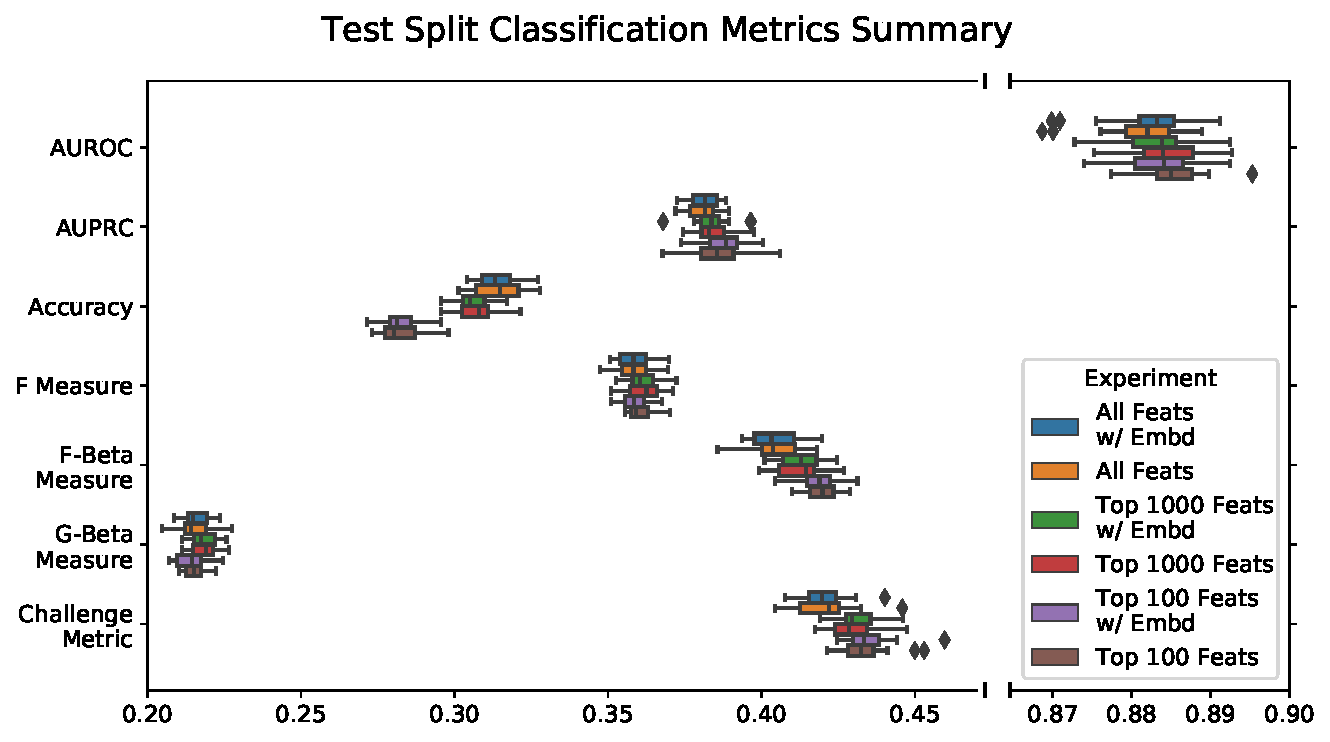
\includegraphics[trim={0.2cm 0.3cm 0.2cm 0.1cm},clip,width=\textwidth]{figure/xgb_aenc_classification_metrics.pdf}
    \caption[Test split classification metrics of XGB ensemble using all engineered features and autoencoder embeddings]{Test split classification metrics of XGB ensemble using 1. All engineered features and autoencoder embeddings; 2. All engineered features; 3. Top 1000 engineered features and autoencoder embeddings per label classifier; 4. Top 1000 engineered features per label classifier; 5. Top 100 engineered features and autoencoder embeddings per label classifier; and 6. Top 100 engineered features per label classifier.}
    \label{fig:xgb_aenc_classification_metrics}
\end{figure}

\begin{table}[t]
    \caption{\label{tab:xgb_aenc_classification_metrics} Test split classification metrics mean ($\bar{x}$) and standard deviations ($\sigma$) for all experiment configurations. Bolded value indicates largest mean for metric category.}
    \vspace{2 mm}
    \centerline{\begin{tabular}{@{}rcccccccc@{}}
    \multirow{2}{*}{\textbf{Experiment}} & & \multirow{2}{*}{\textbf{AUROC}} & \multirow{2}{*}{\textbf{AUPRC}} & \multirow{2}{*}{\textbf{Accuracy}} & \multirow{2}{*}{\textbf{F Measure}} & \multirow{2}{*}{\textbf{F-Beta}} & \multirow{2}{*}{\textbf{G-Beta}} & \textbf{Challenge} \\
    & & & & & & & & \textbf{Metric} \\ \hline
    All Feats & $\bar{x}$ & 0.8821 & 0.3813 & 0.3137 & 0.3587 & 0.4047 & 0.2160 & 0.4207 \\
    w/ Embed & $\sigma$ & $5.3 \times 10^{-3}$ & $5.0 \times 10^{-3}$ & $6.8 \times 10^{-3}$ & $5.9 \times 10^{-3}$ & $8.1 \times 10^{-3}$ & $3.9 \times 10^{-3}$ & $7.7 \times 10^{-3}$ \\ \hline
    \multirow{2}{*}{All Feats} & $\bar{x}$ & 0.8815 & 0.3809 & \textbf{0.3139} & 0.3582 & 0.4036 & 0.2150 & 0.4206 \\
    & $\sigma$ & $5.5 \times 10^{-3}$ & $5.0 \times 10^{-3}$ & $7.9 \times 10^{-3}$ & $6.0 \times 10^{-3}$ & $8.6 \times 10^{-3}$ & $5.2 \times 10^{-3}$ & $1.0 \times 10^{-2}$ \\ \hline
    Top 1000 Feats & $\bar{x}$ & 0.8836 & 0.3837 & 0.3062 & 0.3613 & 0.4128 & \textbf{0.2183} & 0.4316 \\
    w/ Embed & $\sigma$ & $4.8 \times 10^{-3}$ & $6.4 \times 10^{-3}$ & $5.4 \times 10^{-3}$ & $5.4 \times 10^{-3}$ & $6.7 \times 10^{-3}$ & $4.3 \times 10^{-3}$ & $7.0 \times 10^{-3}$ \\ \hline
    \multirow{2}{*}{Top 1000 Feats} & $\bar{x}$ & 0.8843 & 0.3836 & 0.3075 & \textbf{0.3619} & 0.4126 & 0.2179 & 0.4295 \\
    & $\sigma$ & $5.2 \times 10^{-3}$ & $5.6 \times 10^{-3}$ & $6.4 \times 10^{-3}$ & $5.2 \times 10^{-3}$ & $7.5 \times 10^{-3}$ & $4.4 \times 10^{-3}$ & $8.1 \times 10^{-3}$ \\ \hline
    Top 100 Feats & $\bar{x}$ & 0.8836 & \textbf{0.3876} & 0.2820 & 0.3588 & 0.4190 & 0.2143 & \textbf{0.4348} \\
    w/ Embed & $\sigma$ & $4.9 \times 10^{-3}$ & $7.0 \times 10^{-3}$ & $6.2 \times 10^{-3}$ & $5.1 \times 10^{-3}$ & $6.8 \times 10^{-3}$ & $4.9 \times 10^{-3}$ & $7.8 \times 10^{-3}$ \\ \hline
    \multirow{2}{*}{Top 100 Feats} & $\bar{x}$ & \textbf{0.8848} & 0.3857 & 0.2830 & 0.3604 & \textbf{0.4198} & 0.2150 & 0.4335 \\
    & $\sigma$ & $4.5 \times 10^{-3}$ & $8.5 \times 10^{-3}$ & $7.5 \times 10^{-3}$ & $4.0 \times 10^{-3}$ & $5.3 \times 10^{-3}$ & $3.3 \times 10^{-3}$ & $8.2 \times 10^{-3}$ \\
    \end{tabular}}
\end{table}

Refer to Figure~\ref{fig:xgb_aenc_classification_metrics} and Table~\ref{tab:xgb_aenc_classification_metrics} for the test set split classification metric summaries for all experiment configurations.
The experiment configuration with the largest mean challenge score is used the top 100 important features of all engineered features with the autoencoder embeddings.

\begin{figure}[t]
    \centering
    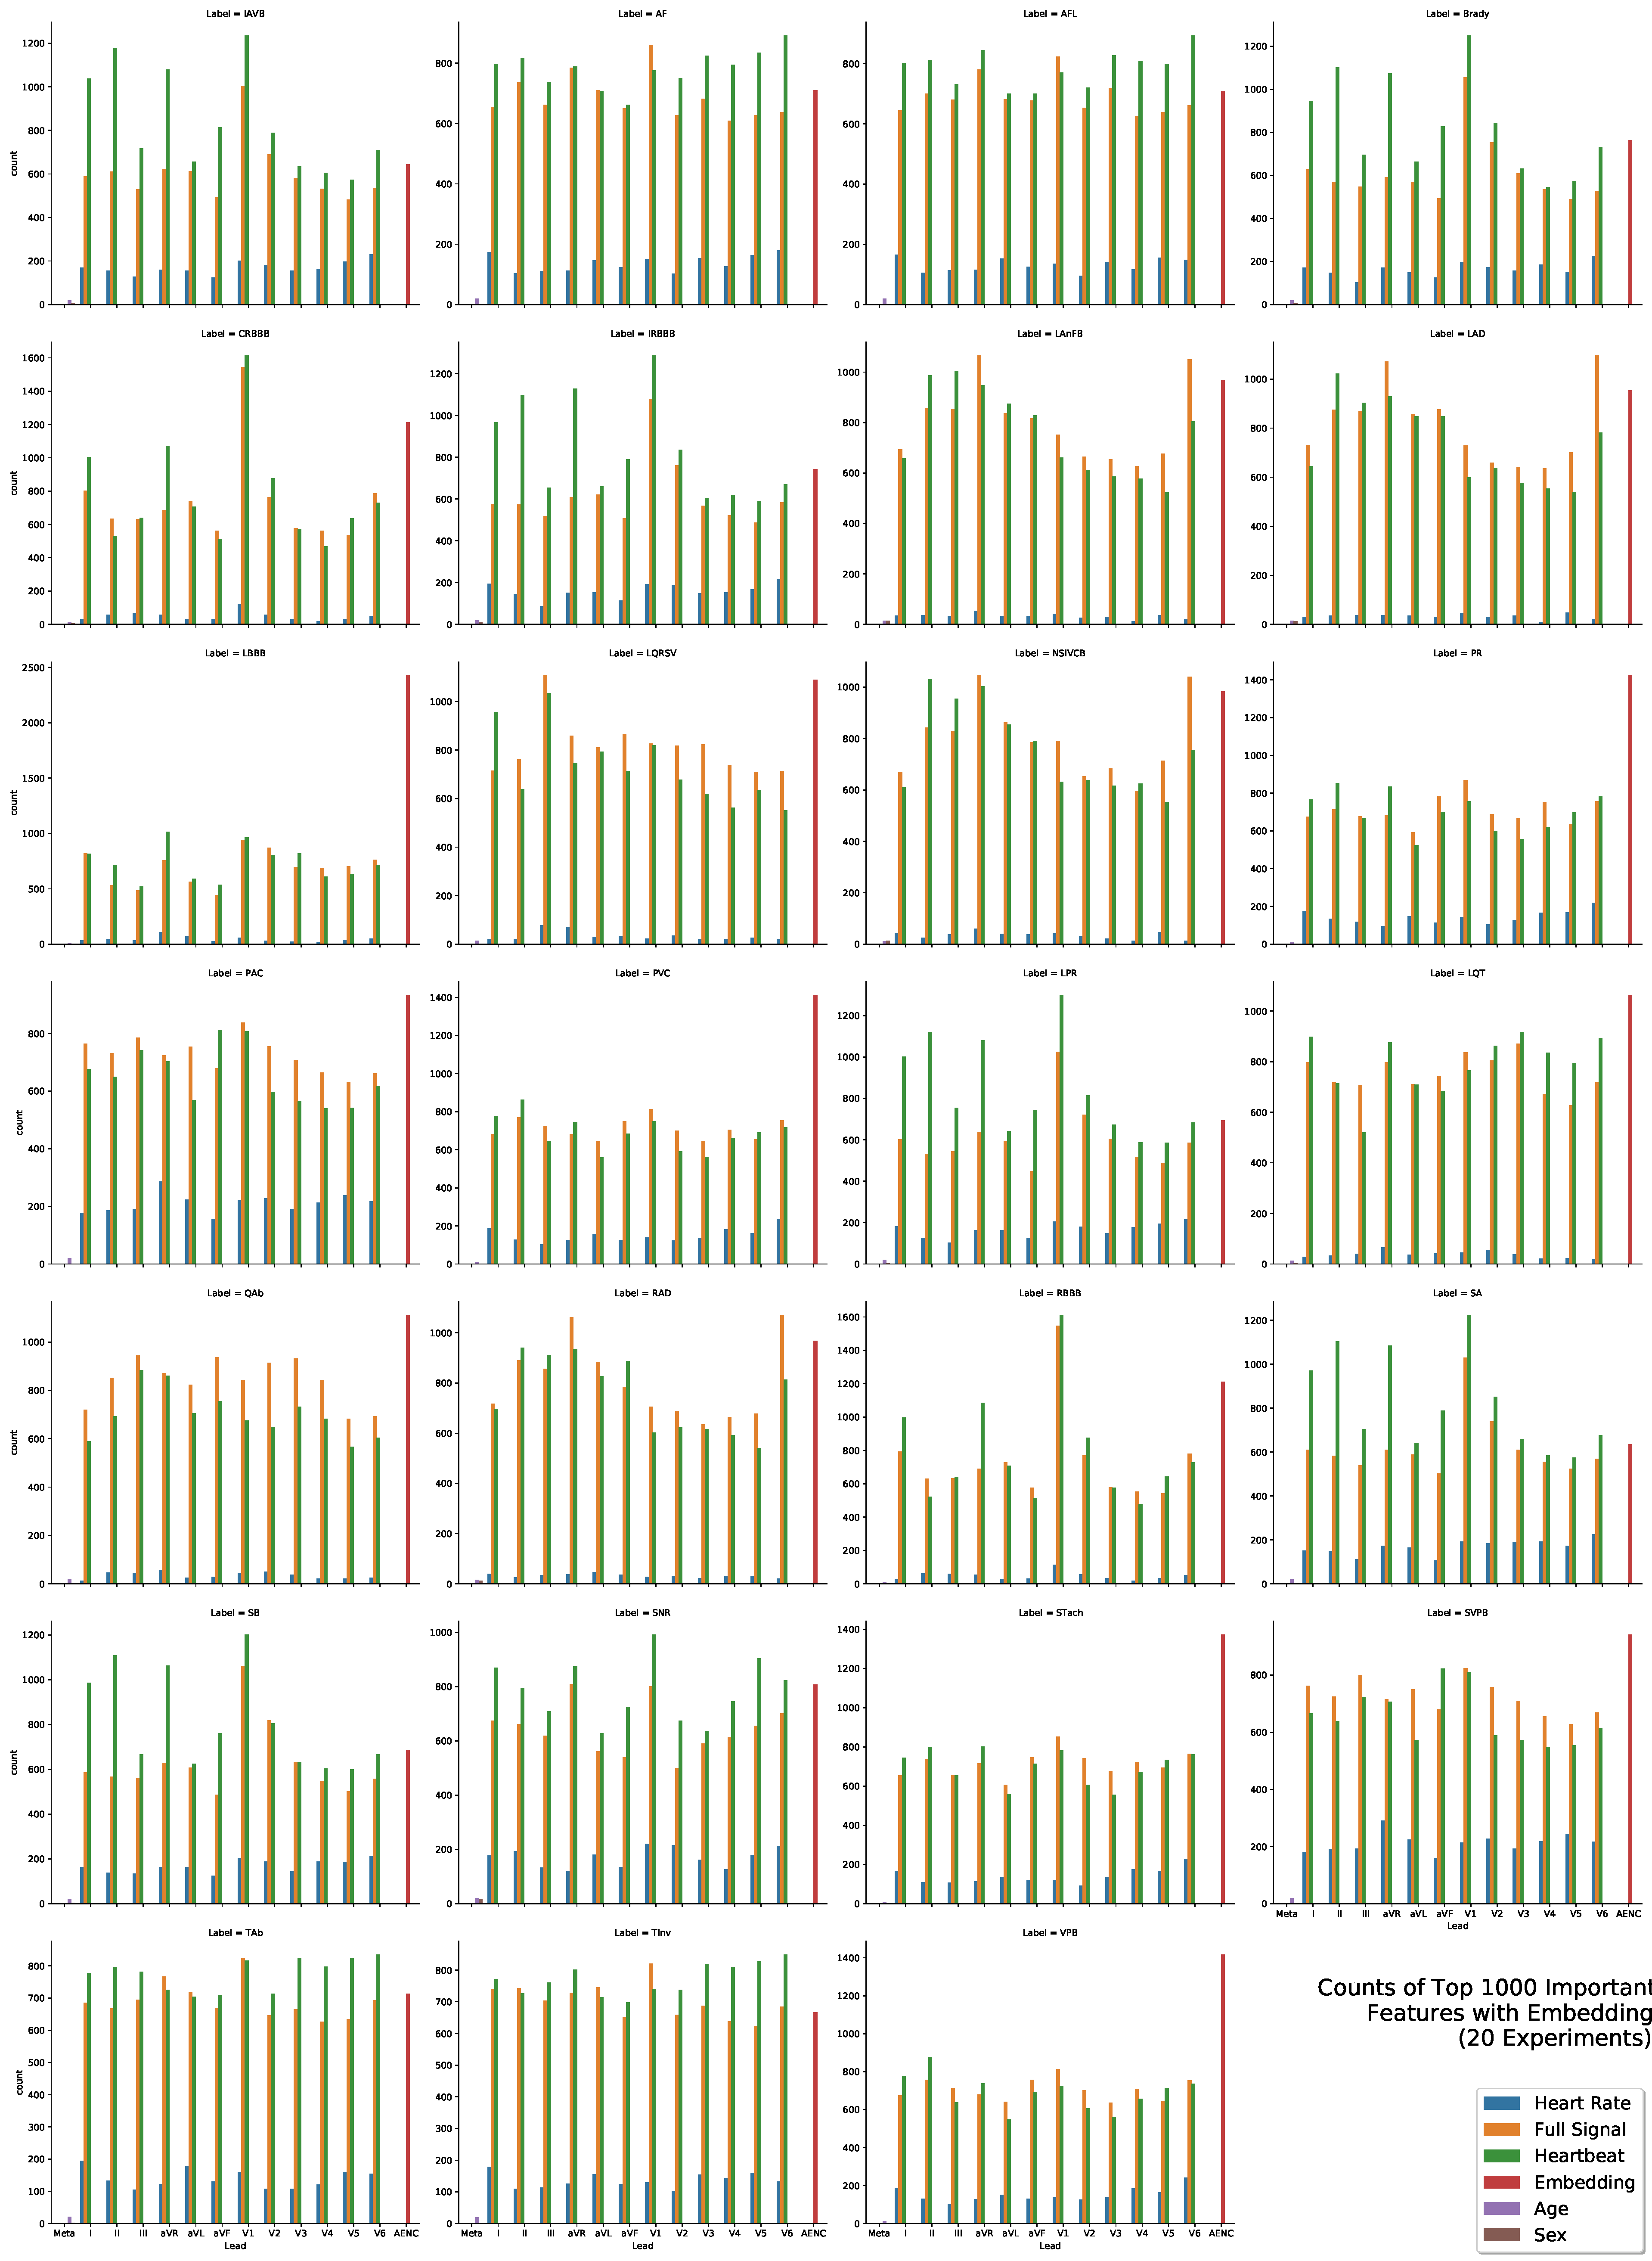
\includegraphics[width=\textwidth]{figure/top_1000_feature_importances_all_w_embedding.pdf}
    \caption{Feature importances of top 1000 features with autoencoder embeddings using an aggregated count over all 20 independent experiments. Each of the 27 diagnosed labels separately displayed, showcasing feature derived lead (or meta/embedding), and category (heart rate, heartbeat, full waveform, embedding, age/sex).}
    \label{fig:xgb_aenc_top_1000_features_labelwise}
\end{figure}

A categorical breakdown of the top 1000 most important features, showcasing label-wise counts of the feature derived lead and category types, can be found in Figure~\ref{fig:xgb_aenc_top_1000_features_labelwise}.

\section{Discussion}
TODO

% Unlike the prior two chapters, the work showcased in this chapter has not been published nor submitted for consideration.
% I acknowledge Dr. Sunil Vasu Kalmady for suggesting the idea of combining my two prior experiments together.
% All other facets are contributed by myself, as I engineered the experiment, generated the relevant figures, and wrote this writeup.

% The takeaways from this chapter are:
% \begin{enumerate}
%     \item Joining the autoencoder embeddings with the manually engineered features to train a set of gradient boosting tree ensemble classifiers resulted in models with poorer classification metrics than using manually engineered features alone.
%     \item Certain labels had increased mean classification $\text{F}_1$ score but none of the label-wise improvements were statistically significant at $p = 0.01$.
%     \item Long term viability of this strategy of combining deep learning techniques with shallow models is not promising, with notable disadvantages: no end-to-end training, unclear model interpretability.
% \end{enumerate}

% \section{Methodology}
% We extend the experiments performed in the manual feature engineering methodology~\cite{wong2020CINC-multilabel-ECG} discussed in Chapter~\ref{chp:xgbensemble} as well as the deep learning approach using the beat to sequence autoencoders~\cite{wong2021ICASSP-multilabel-ECG} discussed in Chapter~\ref{chp:dl_autoenc}.

% We run our corpus of available \gls{ecg} data through the manual feature engineering process to clean and pre-process our signals, then we extract the top 1,000 full waveform, heartbeat template, and heart rate variability features using \emph{tsfresh} and \emph{NeroKit2}.
% Additionally, using the 20 existing and trained beat to sequence autoencoders, we convert our \gls{ecg} records into embeddings of size 768 floating point numbers.
% Our classifier receives \gls{ecg} records as input vectors of size $1,768$.

% We use 20 times repeated random subsampling, keeping identical splits of our \gls{ecg} records as performed in our prior experiments, to mitigate internal validity risk.
% All other XGBoost configuration settings are identical to our previous XGBoost ensemble training experiment, which is discussed in Section~\ref{ssec:xgb_classification}.

% \section{Results}

% \begin{figure}[ht]
%     \centering
%     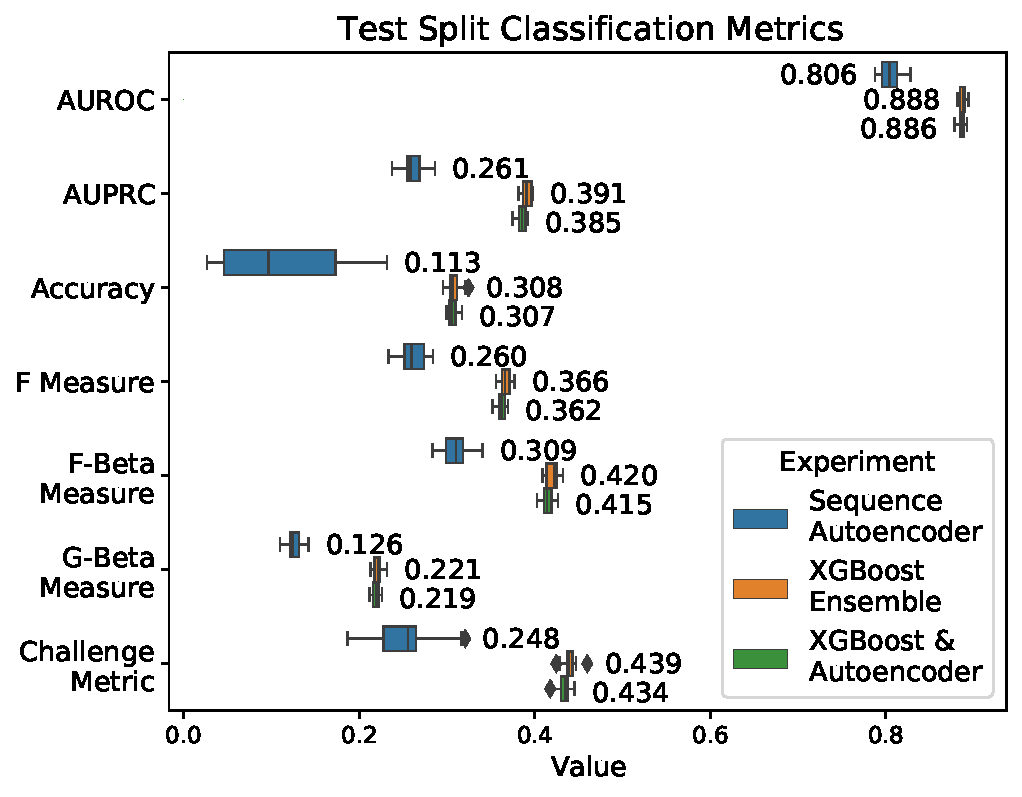
\includegraphics[width=10cm]{figure/classification_metrics_3_way.pdf}
%     \caption[Summary classification metrics comparing gradient boosting decision tree with manual feature engineering, beat to sequence autoencoder classifier, and gradient boosting decision tree with manual feature engineering and autoencoder embeddings.]{Summary classification metrics comparing gradient boosting decision tree with manual feature engineering, beat to sequence autoencoder classifier, and gradient boosting decision tree with manual feature engineering and autoencoder embeddings. Annotations indicate mean value.}
%     \label{fig:joint_xgb_aenc_classification_metrics_summary}
% \end{figure}

% Figure~\ref{fig:joint_xgb_aenc_classification_metrics_summary} contains the summary classification metrics of our original XGBoost methodology~\cite{wong2020CINC-multilabel-ECG}, our beat to sequence autoencoder~\cite{wong2021ICASSP-multilabel-ECG}, and the work discussed in this chapter joining these two approaches together.
% We observe that the additional features derived from the autoencoder caused all classification metrics to decrease respective to using the XGBoost ensemble methodology with manually engineered features alone.

% \begin{figure}[ht]
%     \centering
%     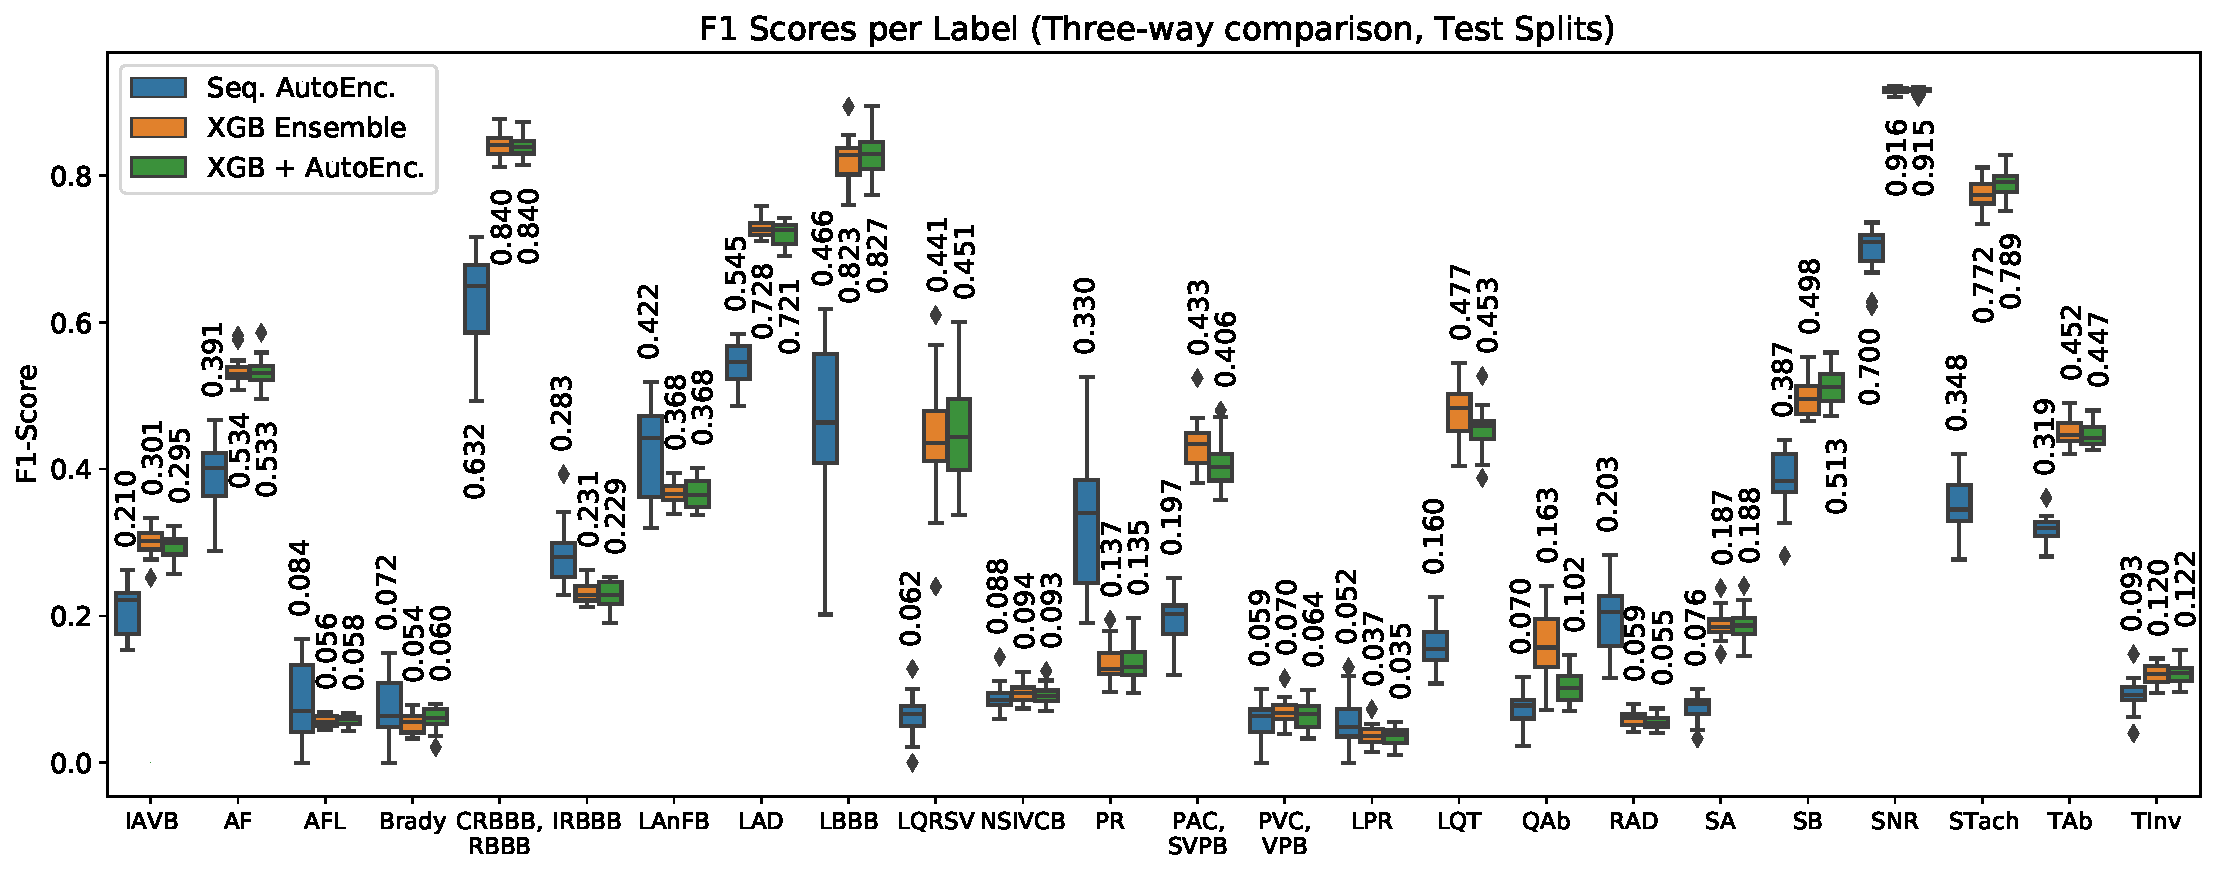
\includegraphics[width=14cm]{figure/label_f1s_3_way.pdf}
%     \caption[Label-wise $\text{F}_1$ scores comparing gradient boosting decision tree with manual feature engineering, beat to sequence autoencoder classifier, and gradient boosting decision tree with manual feature engineering and autoencoder embeddings.]{Label-wise $\text{F}_1$ scores comparing gradient boosting decision tree with manual feature engineering, beat to sequence autoencoder classifier, and gradient boosting decision tree with manual feature engineering and autoencoder embeddings. Annotations indicate mean value.}
%     \label{fig:joint_xgb_aenc_f1_score}
% \end{figure}

% A label-wise comparison of the joint model's $\text{F}_1$ scores compared to our prior work can be found in Figure~\ref{fig:joint_xgb_aenc_f1_score}.
% The Wilcoxon signed rank statistical test is used to compare the XGBoost with autoencoder embedding $\text{F}_1$ scores to the XGBoost without embedding $\text{F}_1$ scores.
% With a $p$-value of $0.01$, none of the labels incurred a statistically significant improvement in $\text{F}_1$ score.

% \section{Discussion}
% In a 2020 panel where Yoshua Bengio discusses current and upcoming deep learning challenges, he dismisses the viability of engineering deep learning models into old-fashioned symbolic machine learning methods, instead proposing learned attention mechanisms as a viable alternative~\cite{2020-yoshua-dlc}.

\end{document}
